% !TEX output_directory=output
%%%%%%%%%%%%%%%%%%%%%%%%%%%%%%%%%%%%%%%%%%%%%%%%%%%%%%%%%%%%%%%%%%%%%%%%%%%%
% !TEX root = main.tex
\documentclass[a4paper,10pt]{article}
\pdfinfo{
     /Title Internationaler Vergleich der Digitalisierung der Krankenhauslandschaft
     /Subject Hauptseminar
     /Author Johannes Wolf
}
\title{Internationaler Vergleich der Digitalisierung der Krankenhauslandschaft:
Treibergrößen und Defizitbereiche in Deutschland}
\author{Johannes Wolf}
\date{\today}

%%%%%%%%%%%%%%%%%%%%%%%%%%%%%%%%%%%%%%%%%%%%%%%%%%%%%%%%%%%%%%%%%%%%%%%%%%%%
% Includes
%%%%%%%%%%%%%%%%%%%%%%%%%%%%%%%%%%%%%%%%%%%%%%%%%%%%%%%%%%%%%%%%%%%%%%%%%%%%
\usepackage[utf8]{inputenc}
\usepackage{csquotes}
\usepackage[german]{babel}
\usepackage[T1]{fontenc}
\usepackage[margin=23mm,bottom=30mm]{geometry}
\usepackage[table,usenames,dvipsnames]{xcolor}
\usepackage{graphicx, wrapfig, helvet, titlesec, fancyhdr}
\usepackage[germankw,german]{algorithm2e}
\usepackage{tikz}
\usepackage{tikz-qtree}
\usepackage{eurosym}
\usetikzlibrary{trees}
\tikzset{
  treenode/.style = {shape=rectangle, rounded corners,
                     draw, align=center},
  root/.style     = {treenode, font=\Large, bottom color=red!30},
  env/.style      = {treenode, font=\ttfamily\normalsize},
  dummy/.style    = {circle,draw}
}
\usepackage{amsmath,amsfonts,amssymb,amsthm}
\usepackage{hyperref} % verwandelt alle Kapitelüberschriften, Verweise aufs Literaturverzeichnis und andere Querverweise in PDF-Hyperlinks
\hypersetup{
	pdftitle={Internationaler Vergleich der Digitalisierung der Krankenhauslandschaft},
	pdfauthor={Johannes Wolf},
	pdfborder={0 0 0} % entfernt hässliche Kästen um Links
}
\usepackage[%
  backend=biber      % biber or bibtex
 ,style=authortitle
 ,citestyle=authoryear-comp %authoryear-icomp
 % ,sorting=none        % no sorting
 ,sorting=nyt         % name, year, title
 ,dashed=false        % so author names aren't replaced by a dash
 ,block=none
 ,indexing=false
 ,citereset=none
 ,isbn=true
 ,url=true
 ,doi=true            % prints doi (digital object identifier)
 ,natbib=true         % if you need natbib functions
 ,language=german
 ,maxcitenames=1			% Cite as 'Name et al.' if there are multiple authors
]{biblatex}
\addbibresource{Quellen.bib}  % better than \bibliography
\DefineBibliographyStrings{german}{
	bibliography = {Literaturverzeichnis},
  andothers = {et al.}
}
\defbibheading{bibliography}[\bibname]{%
	 \noindent\LARGE\textbf{\textcolor{thmgrey}#1}
}

% define color used for titels. Offical color of the thm
\definecolor{thmgrey}{HTML}{4a5c66}
\definecolor{green}{HTML}{4E9A06}

% sets the vspace ahead of a paragraph headline (unnumbered subsection)
\newcommand\parheadvspace{1ex}

% set font to Arial look-alike helvet
\renewcommand{\familydefault}{\sfdefault}

% Defines for mathematical notation. Add additional defines as needed.
\def\O{\mathcal{O}}

% Set paragraph indentation and spacing
\setlength{\parindent}{0pt}
\setlength{\parskip}{0.5ex}

% All this just to have page numbers not centered smh
% \pagestyle{fancy}
% \fancyhf{}
% \renewcommand{\headrulewidth}{0pt}
% \renewcommand{\footrulewidth}{0pt}
% \rfoot{\thepage}

% Reformat section
\titleformat
{\section} % command
[block] % shape
{\LARGE\bfseries\color{thmgrey}} % format
{\thesection} % label
{1ex} % sep between label and title
{} % before-code
{} % after-code

% Reformat subsection
\titleformat
{\subsection} % command
[block] % shape
{\large\bfseries\color{thmgrey}} % format
{\thesubsection} % label
{1ex} % sep between label and title
{} % before-code
{} % after-code

% Reformat subsubsection
\titleformat
{\subsubsection} % command
[block] % shape
{\large\bfseries\color{thmgrey}} % format
{\thesubsubsection} % label
{1ex} % sep between label and title
{} % before-code
{} % after-code
 % packages and global definitions
% !TEX root = main.tex
% Definition of the Cover Page
\def\seminarheader{{
  \pagenumbering{Roman}
  \hypersetup{pageanchor=false}
  \begin{titlepage}
    \pagestyle{empty}
    % header (thm logo)
    \begin{wrapfigure}{r}{0.68\textwidth}
      \centering
      
\includegraphics[width=0.68\textwidth]{Bilder/Logo_THM_FB13.png}
    \end{wrapfigure}
    \parbox[t]{0.32\textwidth}{
      \vspace{-0.5ex}
      \color{thmgrey}
      Hauptseminar\\*
      Dr. Eschenhof-Kammer \\*
      Wintersemester 2020/21 \\*
    }

    % Title of the Paper
    \vspace*{\fill} % hack hack hackedy hack
    \parbox[t]{0.95\textwidth}{
      \center\LARGE\bf\color{thmgrey} 
      Seminararbeit\\*
      \vspace{1ex}
      Internationaler Vergleich der Digitalisierung der Krankenhauslandschaft:\\
Treibergrößen und Defizitbereiche in Deutschland\\*
    }
    \vspace*{\fill}

    % Contact information
    \parbox[t]{\textwidth}{
      \large Johannes Wolf \\*
      \textcolor{thmgrey}{Email:} johannes.wolf@mnd.thm.de \\*
      \textcolor{thmgrey}{Matrikelnummer:} 5146451 \\*
    }
  \end{titlepage}
  % new page
  \hypersetup{pageanchor=true}
  \pagenumbering{Roman}
  \tableofcontents
  \newpage
}}

% Add header to the beginning of the document
\AtBeginDocument{\seminarheader}
 % titelpage and table of contents
%%%%%%%%%%%%%%%%%%%%%%%%%%%%%%%%%%%%%%%%%%%%%%%%%%%%%%%%%%%%%%%%%%%%%%%%%%%%
\begin{document}
%\section*{Abstract}
%\addcontentsline{toc}{section}{Abstract}
%\newpage
\pagenumbering{arabic}
\section{Einleitung}
	\subsection{Was beinhaltet Digitalisierung?}
	\parencite[11]{braeutigam2017}
\section{Das digitale Krankenhaus}
	\begin{itemize}
		\item Beispiele
		\begin{itemize}
			\item "Beispielweise wird Software angeboten, die aufgrund eingespeister Informationen zu einzelnen Patienten Pflegemaßnahmen vorgibt. Im ärztlichen Bereich wird die Standardisierung, Automatisierung und Kontrolle bei chirurgischen Eingriffen thematisiert." \parencite[16]{braeutigam2017}
			\item 
		\end{itemize}
	\end{itemize}
	\subsection{IT-Unterstützung der Behandlung}
	\parencite[51]{oswald2019} \parencite[14]{braeutigam2017}
	\begin{itemize}
		\item Telemonitoring
		\item mHealth
		\item Wearable Computing
		\item Operations-Roboter
	\end{itemize}
	\subsection{IT-Unterstützung der Support- und Managementprozesse/Versorgungsprozesse}
	\parencite{oswald2019} \parencite[14]{braeutigam2017}
	\begin{itemize}
		\item Krankenhausinformationssystem (KIS)
		\item Elektronische Patientenakte (EPA)
		\item Patientendatenmanagement (PDMS)
		\item Labor-Informationssysteme (LIS)
		\item Radiologie-Informationssystem (RIS)
		\item Picture Archiving and Communication System (PACS): Bildarchivierungs- und Kommunikationssystem
		\item Cumputerized Physician Order Entry (CPOE): elektronische Arzneimittelverordnung
		\item WLAN
		\item Location Based Services (Papi)
	\end{itemize}
	\subsection{IT-Unterstützung der klinischen Prozesse}
		\begin{itemize}
			\item Klinische Prozesse
			\begin{itemize}
				\item Aufnahme, Visite, [OP-Vorbereitung, OP-Nachbereitung], Entlassung (ggf. als Grafik) \parencite[37]{huebner2019}
			\end{itemize}
			\item Deskriptoren
		\begin{itemize} 
			\item Information und Daten
			\item IT-Funktionen/Anwendungen
			\item Integration
			\item Distribution
		\end{itemize}
		\item In den Kapiteln \ref{sec:stand in deutschland} und \ref{sec:laendervergleich} wird die Sicht der IT auf die klinischen Prozesse für die Analyse in Deutschland und den Ländervergleich mit Österreich und der Schweiz herangezogen.
		\end{itemize}
	\subsection{IT-Report}
	IT-Report der Uni Osnabrück beschreiben
\section{Bewertungskriterien und Treibergrößen des Digitalisierungsfortschritts}
	\subsection{Kennzahlen}
	\subsubsection{Workflow Composite Score}
		Aufnahme, Visite, [Op-Vorbereitung, Op-Nachbereitung], Entlassung (ggf. als Grafik)\\
		%\begin{figure}[h]
		%	\centering
		%	\includegraphics[width=0.8\textwidth]{Bilder/WCS_Hübner_2018_S22.png}
		%	\caption{Hierachie des Workflow Composite Scores \parencite[22]{huebner2018}}
		%	\label{fig:WCS}
		%\end{figure}
		Diese Kennzahl bedient sich des \textit{Prinzip der klinischen Informationslogistik}. Bei diesem Prinzip "sollte ein [Krankenhausinformationssystem] immer die richtigen Patienteninformation zur richtigen Zeit am richtigen Ort in der richtigen Qualität für die richtigen Personen bereitstellen."\parencite[36]{huebner2019} Der Workflow Composite Score misst inwieweit dieser Standard erreicht ist. Hierbei werden über 100 Einzelindikatoren erfasst und, wenn möglich, in 5 klinische Prozesse (Aufnahme, Visite, OP-Vorbereitung, OP-Nachbereitung, Entlassung) eingeteilt. Bei Krankenhäusern, die nicht über einen OP verfügen, werden nur Aufnahme, Visite und Entlassung betrachtet. Innerhalb dieser Prozesse werden die Indikatoren noch 4 Deskriptoren aufgeteilt. Diese Indikatoren sind
		\begin{enumerate}
			\item Daten und Informationen
			\item Funktionen
			\item Integration und
			\item Distribution.
		\end{enumerate}
		Bei \textit{Daten und Informationen} geht es um die Vielfalt der elektronisch verfügbaren Patienteninformationen. Teil dieses Deskriptors ist z.B. die Frage ob Patientenstammdaten bei der Aufnahme schon in elektronischer Form vorhanden sind oder ob sie erst manuell aufgenommen werden müssen. \textit{Funktion} erfasst welche IT-Anwendungen zur Verfügung stehen, z.B. ein System zur Belegesteuerung, aber auch das Vorhandensein von WLAN. Inwieweit diese Anwendungen miteinander verknüpft sind zeigt der Deskriptor \textit{Integration} auf. \textit{Distribution} sind die Mittel mit denen Informationen an ihre Nutzer gebracht werden. Können Pflegekräfte Patientendaten nur an einem PC einsehen oder gibt es Tablets, die einfacher mit auf ein Zimmer genommen werden können?

		Für die Schnittstelle
	\subsubsection{ICS}
	\subsubsection{PIMCS}
	\subsubsection{EMRAM}
	\parencite{Stephani2019}
	\subsection{Treibergrößen (definieren und gemeinsames Verständnis definieren)}
	\begin{itemize}
		\item Hoffnungen \parencite[15]{braeutigam2017}
		\begin{itemize}
			\item die Verbesserung der Versorgungsqualität
			\item die Erleichterung der Dokumentation
			\item Verbesserung bei Organisation und Kommunikation
			\item Qualitätssteigerungen bei Diagnostik und Therapie, insbesondere bei Operationen
			\item Zeitersparnis
			\item mehr Zeit für den direkten Patientenkontakt vor allem in der Pflege
			\item Entlastung von Routineaufgaben
			\item Entlastung von körperlich anstrengenden Tätigkeiten
			\item Fernbetreuung von Patienten
		\end{itemize}
	\end{itemize}
	\begin{itemize}
		\item Methodik
		\begin{itemize}
			\item Betrachtung des WCS über KH-Attribute (z.B. Trägerschaft)
			\item (mind. 0,05 Signifikanz des Mittelwertunterschieds)
		\end{itemize}
	\end{itemize}
\section{Aktueller Stand der Digitalisierung in deutschen Krankenhäuser} \label{sec:stand in deutschland}
	\subsection{Aktueller Stand bzgl. Bewertungskriterien}
		Veränderung von 2018 zu 2020
	\subsection{Treibergrößen für Digitalisierung in Deutschland}
	\begin{itemize}
		\item Verbundstatus \parencite{cresswell2013}
		\item Lehrstatus
		\item OP
		\item Größe \parencite{cresswell2013}
		\item nicht: Trägerschaft \parencite{cresswell2013}
	\end{itemize}
	\subsection{Defizite / Defizitbereiche}
	\begin{itemize}
		\item IT-Governance
		\item Distribution von Daten (Endgeräte)
		\item Politik-Gedöns
	\end{itemize}
\section{Ländervergleich} \label{sec:laendervergleich}
% !TEX root = ../main.tex
Um die Digitalisierung der deutschen Krankenhauslandschaft im internationalem Vergleich zu sehen, werden hier Deutschland, Österreich und die deutschsprachige Schweiz miteinander verglichen. Datengrundlage des Vergleichs ist der IT-Report Gesundheitswesen 2020 der Hochschule Osnabrück.
\subsection{IT-Report Gesundheitswesen 2020}
Für diesen Ländervergleich wird der IT-Report Gesundheitswesen 2020 herangezogen, in welchem nicht nur deutsche Krankenhäuser, sondern auch Krankenhäuser aus Österreich und der Schweiz, zum Thema Digitalisierung befragt wurden. Die Umfrage fand im Jahr 2017 vom 1.7. bis zum 14.12. statt und bestand aus 87 Fragen, gerichtet an ärztliche und pflegerische Direktoren. Insgesamt wurden 2421 Krankenhäuser angeschrieben, davon 1951 in Deutschland, 260 in Österreich und 211 aus der deutschsprachigen Schweiz \parencite{huebner2020}. Laut statista gab es im Jahr 2017 1942 Krankenhäuser in Deutschland\footnote{https://de.statista.com/statistik/daten/studie/2617/umfrage/anzahl-der-krankenhaeuser-in-deutschland-seit-2000/}, 271 Krankenhäuser in Österreich\footnote{https://de.statista.com/statistik/daten/studie/298568/umfrage/oesterreic-hanzahl-der-krankenhaeuser-seit-1985/} und 281 Krankenhäuser in der Schweiz\footnote{https://de.statista.com/statistik/daten/studie/306939/umfrage/anzahl-der-krankenhaeuser-in-der-schweiz/}. Es wurden also fasst alle Krankenhäuser in den drei Regionen angeschrieben. Antworten kamen aus 608 Krankenhäusern, davon 492 aus Deutschland (Rücklaufquote $25,2\%$), 49 aus Österreich ($18,8\%$), 67 aus der deutschsprachigen Schweiz ($31,8\%$) . Eine Übersicht über diese Zahlen befindet sich in Tabelle \ref{tab:anzahl-krankenhaeuser}. 
\begin{table}[ht]
\begin{center}
	\begin{tabular}{l|c|c|c|l}
		&Angeschrieben&\parbox[c]{13ex}{\centering Krankenhäuser\\ insgesamt}&Antworten&Rücklaufquote\\
		\hline
		Deutschland&$1951$&$1942$&$608$&$25,2\%$\\
		Österreich&$260$&$271$&$49$&$18,8\%$\\
		Schweiz&$211$&$281$&$67$&$31,8\%$\\
	\end{tabular}
\end{center}
\caption{Übersicht über befragte Krankenhäuser}	
\label{tab:anzahl-krankenhaeuser}
\end{table}

TODO Übersicht über Fragen

In der Studie wurde kein intensiver wertender Vergleich durchgeführt. Daher wurde in dieser Arbeit eine eigene Methodik entwickelt.
\subsection{Methodik}
	Da der IT-Report 2020 keinen quantitativen Vergleich der Ergebnisse angibt, wurde eine eigene Vergleichsmethodik entwickelt. Die Daten lagen nicht in Rohform vor und wurden deshalb manuell in eine Tabellenform zurückgeführt. Für die Bewertung wurde für jede Frage das Land ermittelt, welches am besten abgeschnitten hat. Die Ergebnisse der Befragung werden mit vier verschiedenen Darstellungen vorgestellt, die unterschiedlich ausgelesen und bewertet werden müssen. Es gibt \textit{einfache Balkendiagramme}, \textit{Balkendiagramme mit mehreren Teilfragen}, die mit ja oder nein beantwortet wurden, \textit{gestapelte Balkendiagramme} und \textit{Boxplots}.
	\vspace{\parheadvspace}\\
	\textbf{Einfache Balkendiagramme}\\
	Für Balkendiagramme wurden die Werte der einzelnen Balken in eine Tabelle übernommen. Um die Fragen miteinander zu vergleichen wurde hier entschieden welche Antworten einen positiven Effekt auf Digitalisierung anzeigen. Die Prozentwerte dieser Antworten wurden dann addiert und das Land mit dem höchsten Wert wurde als am besten eingeschätzt.
	\vspace{\parheadvspace}\\
	\textbf{Balkendiagramme mit mehreren Teilfragen}\\
	Für jede Teilfrage wurde die positive Antwort aufgeschrieben.	Fragen, die in dieser Darstellung präsentiert wurden, ermitteln welche IT-Funktionen, Geräte o.Ä. im Krankenhaus zur Verfügung steht. Dabei wird nur die Existenz erfragt. Es wird angenommen, das eine Existenz immer positiv im Hinblick auf die Digitalisierung zu bewerten ist. Unter dieser Annahme wurde für jede Teilfrage ermittelt welches Land am besten ist und die Frage dann dem Land zugeschrieben, das am meisten Teilfragen gewonnen hat. Bei einem Gleichstand von zwei Ländern wurde die Frage für Beide gewertet. Bei einem Gleichstand von allen drei Ländern wurde die Frage ignoriert.
	\vspace{\parheadvspace}\\
	\textbf{Gestapelte Balkendiagramme}\\
	Bei dieser Darstellung haben die Autoren der Studie aus ästhetischen Gründen Angaben unter 10\% nicht als Zahl angezeigt \parencite[298]{huebner2020}. Bei einer hohen Anzahl an Antworten (einem hohen n) wurden die Werte in diesen Fällen geschätzt. Bei einer kleinen Anzahl an Antworten ($n<50$), war die Anzahl der möglichen Werte so gering, das der genaue Wert ermittelt werden konnte. Auch hier besteht jede Frage aus mehreren Teilfragen. Diese werden wie bei den simpleren Balkendiagrammen einzeln einem Land gutgeschrieben und das Land mit den meisten Teilfragen wird dann als Gewinner der Frage gewertet.

	Die Antwortmöglichkeiten auf die Teilfragen haben hier immer eine klare bewertende Reihenfolge. Es geht entweder um Zustimmung mit einer Aussage (\glqq Stimme überhaupt nicht zu\grqq{ }bis \glqq Stimme voll zu\grqq) oder um die Durchdringung einer IT-Funktion (0\%, unter 50\%, über 50\% oder 100\%). \glqq Weiß nicht\grqq{ }wurde ignoriert. Jeder dieser Antwortmöglichkeiten wurde nun eine Wertung von -2 bis 2 zugeschrieben. Jede Wertung wurde mit dem entsprechenden Prozentwert multipliziert und dann aufsummiert. Dem Land mit der höchsten Summe wurde die Teilfrage gutgeschrieben.
	\vspace{\parheadvspace}\\
	\textbf{Boxplots}\\
	Boxplots haben eine sehr hohe Informationsdichte, die allerdings schwer zu vergleichen ist. Daher wurden hier nur die Mediane notiert und miteinander verglichen. Wie bei den vorherigen beiden Darstellungen, gibt es pro Frage mehrere Teilfragen, die wieder einzeln für ein Land entschieden werden, um dann die gewonnen Teilfragen zusammenzuzählen und die Frage dem Land zuzurechnen, das am meisten Teilfragen gewonnen hat.

	Um abschließend eine Übersicht zu gewinnen, werden für jedes Land die Anzahl der gewonnen Fragen berechnet. Zusätzlich werden noch Zwischensummen für die einzelnen klinischen Prozesse gebildet. Jede Frage wird gleich gewichtet. 

% \begin{itemize}
% 	\item Ablesemethodik
% 	\begin{itemize}
% 		\item Bei gestapelten Säulen wurden Werte unter 10\% nicht dazu geschrieben, deshalb wurden sie für große n geschätzt. Für kleine Anzahl der Grundgesamtheit konnten die fehlenden Werte ermittelt werden, da nicht viele in Frage kamen.
% 	\end{itemize}
% 	\item Einfache Vergleichsmethodik
% 	\item Fokus: Universitätsmedizin wird ignoriert
% 	\item Für jede Frage gibt es einen Gewinner
% 	\begin{itemize}
% 		\item Bei Gleichstand von 2 Ländern zählen beide als Gewinner
% 	\end{itemize}
% 	\item Wann ist jemand ein Gewinner?
% 	\item \textit{Weiß nicht} wird ignoriert
% 	\begin{itemize}
% 		\item wird indirekt neutral oder negativ bewertet
% 	\end{itemize}
% 	\item bsp Papier einscannen: Geht das direkt in ne datenbank? Wahrschienlich nicht
% 	\begin{itemize}
% 		\item Boxplots
% 		\item Boxplots erklären \parencite[44]{kronthaler2016}
% 		\begin{itemize}
% 			\item Größter Median > größtes oberstes Quartil > größter oberster Whisker
% 			\item evtl. wie bei Güte der Informationsversorgung
% 		\end{itemize}
% 		\item Einfache Säulen mit wenig Antwortmöglichkeiten
% 		\begin{itemize}
% 			\item Summe der Antworten, die Digitalisierung anzeigen
% 			\item Größte Summe gewinnt
% 		\end{itemize}
% 		\item Ja/Nein Säulen mit vielen Kategorien
% 		\begin{itemize}
% 			\item Jede Kategorie gewinnt einzeln
% 			\item Land mit den meisten Kategorien gewinnt Frage
% 			\item Was passiert wenn Länder gleich viele Kategorien gewinnen
% 		\end{itemize}
% 		\item Gestapelte Säulen
% 		\item Güte der Informationsversorgung (Schweiz hat bei Aufnahme nicht teilgenommen)
% 		\begin{itemize}
% 			\item Antworten werden gewichtet
% 			\item ''Stimme überhaupt nicht zu'' = -2 bis ''Stimme voll zu'' = +2
% 			\item multipliziert mit Prozent der Stimmen und dann addiert
% 			\item Scores für alle Kategorien summieren
% 			\item höchster Score gewinnt
% 		\end{itemize}
% 	\end{itemize}
% 	\item Jeder Prozess wird einzeln betrachtet
% 	\item Für jede Frage wird entschieden was einen Digitalisierungsfortschritt darstellt
% \end{itemize}
\subsection{Gegenüberstellung der Länder}
\begin{figure}
	\centering
	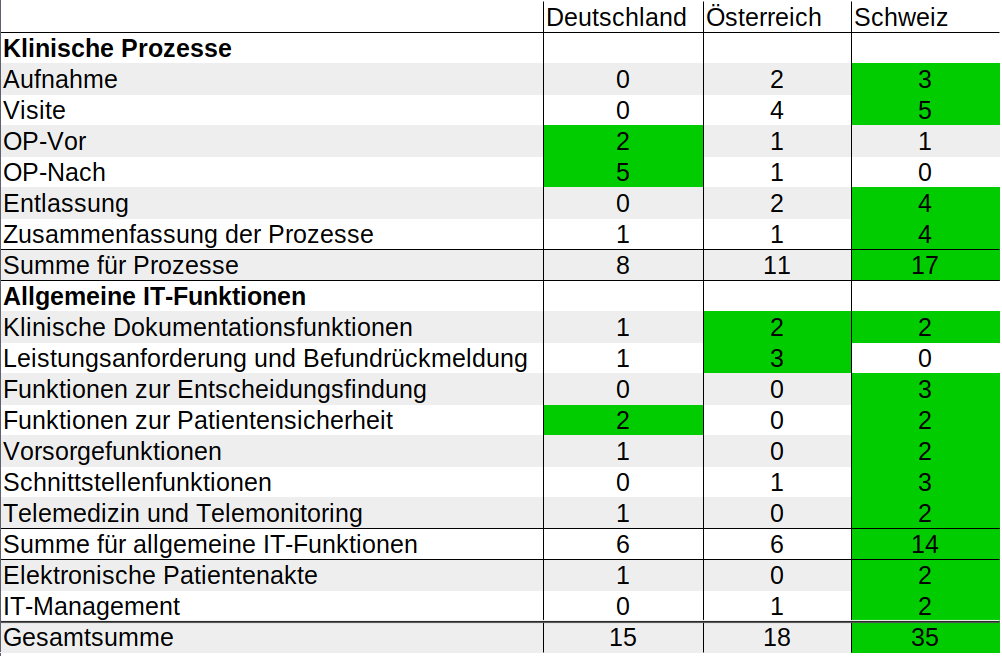
\includegraphics[width=0.7\textwidth]{Bilder/laendervergleich_ergebnisse.png}
	\caption{Ergebnisse des Ländervergleichs. Die Gewinner einer Kategorie sind grün markiert}
	\label{fig:laender_ergebnisse}
\end{figure}
Bei der gewählten Methodik ist zwar erkennbar welches Land die meisten Fragen gewonnen hat, aber nicht wie stark. Diese Ergebnisse geben also nur eine vergleichende und keine Qualitative Übersicht. Die Gegenüberstellung erfolgt nach der Struktur, die im IT-Report Gesundheitswesen 2020 vorgegeben ist. So werden zuerst die klinischen Prozesse betrachtet und anschließend verschiedene IT-Funktionstypen und das IT-Management. Eine Übersicht über die Ergebnisse befindet sich in Abbildung \ref{fig:laender_ergebnisse}.
\vspace{\parheadvspace}\\
\textbf{Klinische Prozesse}\\
In den Prozessen Aufnahme, Visite und Entlassung ist die Schweiz Vorreiter, während in den Unterstützungsprozessen des OP Deutschland führt. Es scheint, dass die externen Schnittstellen, Aufnahme und Entlassung, in Österreich und der Schweiz deutlich digitaler sind als in Deutschland. In der Visite zeigt sich vor allem eine höhere Verfügbarkeit von mobilen Geräten zum Zugriff auf Patientendaten und damit verbunden eine weitere Verbreitung von WLAN in Österreich und der Schweiz im Vergleich zu Deutschland. Daten im OP-Verlauf stehen in Deutschland jedoch deutlich häufiger in elektronischer Form bereit und die Informationsgüte ist höher, was sich am guten Abschneiden in der OP-Vorbereitung widerspiegelt. Bei der OP-Nachbereitung ergibt sich ein ähnliches Bild. Da OP-Daten in deutschen Krankenhäusern häufiger elektronisch verfügbar sind, können sie auch einfacher auf die Stationen übernommen werden. Die Zufriedenheit mit dem IT-Einsatz in den fünf Prozessen ist in der Schweiz am höchsten. Auch die Verfügbarkeit wesentlicher Patientendaten wird von schweizer Klinikern am besten eingeschätzt.
\vspace{\parheadvspace}\\
\textbf{Weitere IT-Funktionen}\\
Das Bild von der Schweiz als Vorreiter verdeutlicht sich bei der Betrachtung ausgewählter IT-Funktionen, die nicht klar einem klinischen Prozess zugeordnet werden. Lediglich bei \textit{Leistungsanforderung und Befundrückmeldung} schneidet Österreich besser ab. Während \textit{Funktionen zur Entscheidungsfindung} in Krankenhäusern aller drei Länder selten eingesetzt werden, sind diese in der Schweiz dennoch am verbreitetsten.
\vspace{\parheadvspace}\\
\textbf{Elektronische Patientenakte}\\
Während eine elektronische Patientenakte (ePA) in nur rund der Hälfte aller deutschen und österreicher Krankenhäuser zur Verfügung steht, haben über drei viertel aller Krankenhäuser in der deutschsprachigen Schweiz eine ePA implementiert. Wenn ein Krankenhaus eine ePA nutzt wird sie meistens im allen relevanten Einheiten genutzt.
\vspace{\parheadvspace}\\
\textbf{IT-Management}\\
Die Zufriedenheit mit dem IT-Support ist in Österreich und der Schweiz höher als in Deutschland. Zusätzlich ist die Integration der IT-Abteilung in der Schweiz am besten, wo es eine hohe Beteiligung des klinischen Personals an IT-Angelegenheiten gibt.

Im Allgemeinen ergibt sich bei Betrachtung der Daten des IT-Report Gesundheitswesen 2020 ein klares Bild: Die deutschsprachige Schweiz ist in Sachen Digitalisierung den andern Ländern vorraus, während Deutschland ehr Schlusslicht ist. Österreich befindet sich im Mittelfeld, ist aber deutlich näher an Deutschland als an der Schweiz. Das ist auch die Einschätzung in der Zusammenfassung des Report \parencite[29]{huebner2020}.

\subsection{Weitere Länder}
\begin{figure}[ht]
	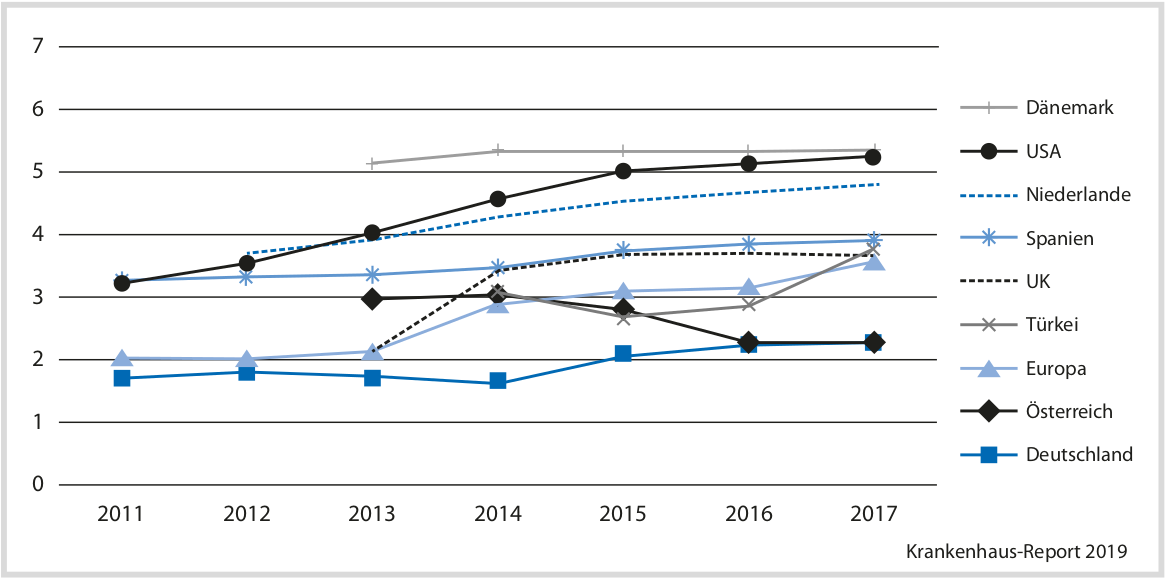
\includegraphics[width=0.95\textwidth]{Bilder/laendervergleich_EMRAM_Stephani_2019.png}
	\caption{Durchschnittliche EMRAM-Werte in ausgewählten Regionen seit 2011 \parencite{Stephani2019}}
	\label{fig:andere_laender}
\end{figure}
Für eine breitere Übersicht über den internationalen Stand der Digitalisierung an Krankenhäusern wird hier eine Übersicht des Schnitts der EMRAM Werte ausgewählter Länder von 2011 bis 2017 (siehe Abbildung \ref{fig:andere_laender}) aus \cite{Stephani2019} herangezogen. Eine Übersicht darüber wie diese Werte ermittelt werden befindet sich in Kapitel \ref{sec:EMRAM}. Es ist zu erkennen, dass Deutschland und Österreich mit einem Mittelwert von $2,3$ auf einem ähnlichen Niveau liegen, das deutlich unter dem europäischen Durchschnitt von $3,6$ liegt. Es gilt hier zu erwähnen, dass sich 167 deutsche Krankenhäuser über den Zeitraum zertifizieren lassen haben während es in Österreich nur 18 waren. Führende Länder in Europa sind die Niederlande ($n=36$) und Dänemark ($n=24$), mit einem jeweiligen Schnitt von $4,8$ und $5,4$. Die Türkei ($n=682$), das vereinigte Königreich($n=105$) und Spanien ($n=156$) liegen nahe am europäischen Mittel.


\section{Fazit und Ausblick}
\begin{itemize}
	\item Treibergröße Geld
\end{itemize}
\newpage
\pagenumbering{Roman}
\setcounter{page}{3}
\printbibliography
\addcontentsline{toc}{section}{Literaturverzeichnis}
\end{document}
